\section{How well it does: toy targets and tabular data}\label{sec:results-toy}

This section compares v3 with every reference on the Boolean toy suites (\cref{sec:res-dlheld7,sec:res-toy-all,sec:res-toy-fail}) and on the 26 tabular datasets (\cref{sec:res-tabular}); \cref{app:further} has the in-sample detail, and \cref{sec:results-img} the image sets. Numbers come from \repo{study/part10/LEARNER_RESULTS.json} unless another file is named, and \cref{app:repro} says which result files stand for v3 and v2. The verdict rules are those of \cref{sec:metrics}, and the discrete learners see the inputs permuted afresh in every fit.

% ------------------------------------------------------------------------------------------------------------------
\subsection{The held-out suite \code{dlheld7}}\label{sec:res-dlheld7}

\code{dlheld7} is the only toy suite held out for v3. It has 12 targets, a fresh draw (seed 70707) from the blind family (\cref{sec:tasks}), and it was fixed in a commit before any Part 10 design work. No result of a Part 10 learner on it was read before v3 was frozen (\cref{sec:discipline}). \Cref{tab:dlheld7} gives every target's definition and $\nstar$.

\begin{table}[t]
\centering{\footnotesize\setlength{\tabcolsep}{3pt}\renewcommand{\arraystretch}{1.15}
\begin{tabularx}{\linewidth}{l>{\raggedright\arraybackslash}Xrrrrrrrr}
\toprule
target & definition & v3 & v2 & \code{nets_wd} & \hd{\code{nets_}\\\code{cewd0.3}} & \hd{\code{nets_}\\\code{cewd1.0}} & \code{nets_best} & \code{lin} & \code{hgb}\\
\midrule
f7\_00 & {\scriptsize OR([|s1| $\le$ 0],\allowbreak{} [s2 == $-$1]),\allowbreak{} s1 = x1+\allowbreak{}x2\allowbreak{}$-$x3\allowbreak{}$-$x4,\allowbreak{} s2 = $-$x5\allowbreak{}$-$x6\allowbreak{}$-$x7+\allowbreak{}x8+\allowbreak{}x9+\allowbreak{}x10+\allowbreak{}x11} & 203 & 207 & 2418 & 1545 & 1565 & 1545 & never & 6208\\
f7\_01 & {\scriptsize [s $\le$ 1],\allowbreak{} s = x1+...+\allowbreak{}x13} & 106 & 107 & 205 & 121 & 119 & 119 & 111 & 684\\
f7\_02 & {\scriptsize OR(AND(x2,\allowbreak{}$-$x6,\allowbreak{}$-$x8),\allowbreak{} AND(x1,\allowbreak{}$-$x2,\allowbreak{}$-$x4,\allowbreak{}$-$x5),\allowbreak{} AND(x3,\allowbreak{}$-$x5,\allowbreak{}$-$x7))} & 106 & 106 & 337 & 341 & 348 & 337 & never & 120\\
f7\_03 & {\scriptsize $-$x11 ? [((s1+6)/2) mod 4 != 2] : [|s2| > 2],\allowbreak{} s1 = x1+...+\allowbreak{}x6,\allowbreak{} s2 = x7+...+\allowbreak{}x10} & 352 & 342 & 1710 & 1665 & 1599 & 1599 & never & 2199\\
f7\_04 & {\scriptsize if AND($-$x6,\allowbreak{}$-$x9) $\to$ +1; elif $-$x8 $\to$ $-$1; elif $-$x4 $\to$ +1; elif $-$x2 $\to$ $-$1; elif x7 $\to$ $-$1; elif x5 $\to$ $-$1; elif AND(x3,\allowbreak{}x1) $\to$ $-$1; else +1} & 70 & 74 & 164 & 175 & 181 & 164 & never & 84\\
f7\_05 & {\scriptsize [((s+14)/2) mod 3 != 0],\allowbreak{} s = x1+...+\allowbreak{}x14} & never & never & never & never & never & never & never & never\\
f7\_06 & {\scriptsize OR(AND(AND($-$x1,\allowbreak{}x2),\allowbreak{}AND(AND($-$x3,\allowbreak{}x4),\allowbreak{}$-$x5)),\allowbreak{}AND(OR($-$x6,\allowbreak{}x7),\allowbreak{}x8))} & 44 & 43 & 108 & 124 & 124 & 108 & 127 & 59\\
f7\_07 & {\scriptsize [$-$2 $\le$ s $\le$ 8] * x13,\allowbreak{} s = $-$x1+\allowbreak{}x2\allowbreak{}$-$x3+\allowbreak{}x4+\allowbreak{}x5+\allowbreak{}x6+\allowbreak{}x7+\allowbreak{}x8\allowbreak{}$-$x9+\allowbreak{}x10\allowbreak{}$-$x11+\allowbreak{}x12} & 174 & 174 & 445 & 443 & 415 & 415 & never & 1373\\
f7\_08 & {\scriptsize [s in \{$-$11,\allowbreak{}$-$9,\allowbreak{}$-$3,\allowbreak{}1,\allowbreak{}9,\allowbreak{}11\}],\allowbreak{} s = x1+...+\allowbreak{}x11} & 634 & 634 & 5843 & 3239 & 2932 & 2932 & never & never\\
f7\_09 & {\scriptsize [s $\le$ 0] * x11 * x12,\allowbreak{} s = x1\allowbreak{}$-$x2+\allowbreak{}x3\allowbreak{}$-$x4+\allowbreak{}x5\allowbreak{}$-$x6+\allowbreak{}x7+\allowbreak{}x8+\allowbreak{}x9+\allowbreak{}x10} & 215 & 215 & 1000 & 883 & 928 & 883 & never & never\\
f7\_10 & {\scriptsize [u $\le$ $-$1],\allowbreak{} u = s + 2*(x6),\allowbreak{} s = x1+...+\allowbreak{}x5} & 82 & 82 & 210 & 120 & 119 & 119 & 87 & 114\\
f7\_11 & {\scriptsize $-$x11 ? [s1 in \{$-$4,\allowbreak{}4\}] : [|s2| $\le$ 4],\allowbreak{} s1 = x1+\allowbreak{}x2\allowbreak{}$-$x3+\allowbreak{}x4,\allowbreak{} s2 = $-$x5\allowbreak{}$-$x6+\allowbreak{}x7\allowbreak{}$-$x8\allowbreak{}$-$x9+\allowbreak{}x10} & 55 & 55 & 114 & 144 & 141 & 114 & 119 & 63\\
\bottomrule
\end{tabularx}
}
\caption{The held-out toy suite \code{dlheld7}: $\nstar$, the training-set size at 10\% test error (mean of 3 seeds, interpolated in $\log n$), for v3, v2, the three pre-registered network variants, their per-target minimum \code{nets_best}, and the calibration references \code{lin} and \code{hgb} \status{Numerical}. v3 and v2 see the inputs permuted per fit. ``never'': 10\% error is not reached by $n=16384$. In the definitions, $[\cdot]$ is $+1$ when the condition holds and $-1$ otherwise; \texttt{*} multiplies $\pm1$ values; \texttt{c ? a : b} is a multiplexer ($a$ when $c=+1$); a literal \texttt{x5} or \texttt{$-$x5} inside AND/OR, a decision-list rule or a selector stands for $x_5=+1$ or $x_5=-1$. f7\_02, f7\_04 and f7\_06 are the family's non-symmetric controls. Source: \repo{study/part10/LEARNER_RESULTS.json}.}
\label{tab:dlheld7}
\end{table}

\paragraph{Against the networks} \status{Numerical}.
\begin{itemize}
\item \emph{Against \code{nets_best}:} mean $\log_2\nstar$ ratio $-1.50$ over the 11 targets that both learn, about $2.8\times$ less data. v3 is clearly better on 10 of 12 targets and clearly worse on none. The 11 per-target ratios have s.d.\ 0.80; treating the targets as independent draws from the family, the mean has a standard error of about 0.24.
\item \emph{The two that are not wins.} f7\_01, a threshold of a 13-input count, is a tie: 106 against 119. f7\_05, a residue class mod 3 of a 14-input count, is learned by no learner (\cref{sec:res-toy-fail}).
\item \emph{Against each variant alone:} $-1.83$ against \code{nets_wd} (11 of 12 targets clearly better), $-1.59$ against \code{nets_cewd0.3} (10 of 12) and $-1.58$ against \code{nets_cewd1.0} (10 of 12). No variant is clearly better than v3 on any target.
\item \emph{Largest margins.} f7\_00, an OR of conditions on two signed sums: 203 against 1545 ($\log_2$ ratio $-2.93$). f7\_08, an arbitrary accept set of an 11-input count: 634 against 2932. f7\_03, a multiplexer between a residue class mod 4 of a 6-input count and a condition on $|s|$ for a 4-input count $s$: 352 against 1599. f7\_09, a threshold of a signed 10-input sum times the parity $x_{11}x_{12}$: 215 against 883.
\item \emph{Smallest margins.} The two halfspaces: f7\_01 (106 against 119) and f7\_10, $[x_1+\dots+x_5+2x_6\le-1]$ (82 against 119).
\end{itemize}

\paragraph{Which wins need no feature search} \status{Numerical}. \code{lin} reaches 10\% error on only 4 of the 12 targets, and \code{hgb} on 9. v3's mean $\log_2$ ratio is $-0.70$ against \code{lin} (over those 4) and $-1.64$ against \code{hgb} (over those 9); it is clearly better than \code{hgb} on 9 targets and than \code{lin} on 9, and clearly worse than neither on any. The wins over the networks fall into two groups.
\begin{itemize}
\item \emph{Five wins need no feature search.} A learner that searches no features is already clearly better than \code{nets_best} on five targets: \code{hgb} on the three controls (f7\_02, a DNF; f7\_04, a decision list; f7\_06, a read-once formula) and on the multiplexer f7\_11, and \code{lin} on the halfspace f7\_10. On these five, v3 is ahead of the better calibration reference by factors of 1.06--1.35 only ($\log_2$ ratios $-0.09$ to $-0.43$).
\item \emph{Five wins need the feature search.} On the other seven targets neither \code{lin} nor \code{hgb} beats the networks. \code{hgb} needs 684--6208 samples or never reaches 10\%, and \code{lin} learns only f7\_01. There v3's mean against \code{nets_best} is $-1.80$: clearly better on 5 (f7\_00, f7\_03, f7\_07, f7\_08, f7\_09, all sum-structured), a tie on f7\_01, and f7\_05 learned by none.
\end{itemize}

\paragraph{Against v2} \status{Numerical}. The mean $\log_2\nstar$ ratio is $-0.004$. No target is clearly better or worse, and the largest per-target change is $0.09$ in $\log_2$ (f7\_04: 70 against 74). So the Part 10 toy component changes nothing measurable on the held-out suite. The best-learner rule only asked that v3 not be worse than v2 there (mean $\le+0.1$). v3 became the learner of this paper through its image side (\cref{sec:results-img}). Over all 138 toy targets, v3's $\nstar$ differs clearly from v2's on 14, 12 lower and 2 higher, none of them on \code{dlheld7}; \cref{app:further-v2v3} lists them with what the models show.

\paragraph{Why nothing moved on \code{dlheld7}} \status{Heuristic}. The gains of v1.3 are concentrated on a few targets: 12 of 138, 11 of which v3 now learns at $n\le256$. A 12-target draw can easily contain none of them. The three draws of the blind family agree with this: v3's mean against v2 is $-0.05$ on \code{dlfamdev} (development), $-0.25$ on \code{dlheld6} (used by the builder) and $-0.004$ on \code{dlheld7}. \code{dlheld7} has one weighted-sum target, f7\_10. It is a halfspace that v2 already learns at the same $\nstar$ (82), although at $n=256$ only v3's model holds the exact weighted block.

\paragraph{Compute} \status{Numerical}. Every v3 fit on \code{dlheld7} used at most 0.53 of one network training run's FLOPs (f7\_04). Over all 11 suites (every v3 toy fit) the maximum is 0.83 (h5s7 on \code{dlheld5}). CPU time per fit is at most 46\,s on the shared 4-core machine (\code{designed}, thr10). Source: the \texttt{flops} and \texttt{cpu\_seconds} fields of the v3 result files.

% ------------------------------------------------------------------------------------------------------------------
\subsection{Every toy suite}\label{sec:res-toy-all}

\begin{table}[t]
\centering{\footnotesize\setlength{\tabcolsep}{4pt}
\begin{tabular}{llccccc}
\toprule
suite & status & targets & v3 vs \code{nets_best} & v3 vs v2 & v3 vs \code{lin} & v3 vs \code{hgb}\\
\midrule
\code{designed} & dev & 21 & $-2.42$ (21/0) & $-0.03$ (1/0) & $-0.85$ (19/0) & --\\
\code{random} & dev check & \multicolumn{5}{c}{(not run)}\\
\code{dlheld} & held out (P6) & \multicolumn{5}{c}{(not run)}\\
\code{dlheld2} & held out (P6) & 7 & $-1.99$ (7/0) & $-0.14$ (1/0) & $-0.58$ (5/0) & $-2.79$ (6/0)\\
\code{dlheld3} & held out (P8) & 10 & $-1.80$ (10/0) & $-0.04$ (0/0) & $-0.99$ (9/0) & $-1.82$ (9/0)\\
\code{dlsymdev} & dev (P9) & 8 & $-2.22$ (8/0) & $-0.18$ (2/0) & n/a (8/0) & --\\
\code{dlheld4} & held out (P9)$^a$ & 12 & $-1.87$ (12/0) & $-0.19$ (3/0) & $-1.54$ (12/0) & $-2.85$ (11/0)\\
\code{dlheld5} & held out (P9) & 12 & $-2.44$ (10/0) & $-0.04$ (1/0) & n/a (11/0) & $-4.11$ (11/0)\\
\code{dlheld6} & held out (P9), dev (P10)$^b$ & 12 & $-1.50$ (11/1) & $-0.25$ (2/0) & $-1.13$ (11/0) & $-2.21$ (10/0)\\
\code{dlfamdev} & dev (P10) & 12 & -- & $-0.05$ (1/1) & -- & --\\
\code{dlheld7} & \textbf{held out (P10)} & 12 & $-1.50$ (10/0) & $-0.00$ (0/0) & $-0.70$ (9/0) & $-1.64$ (9/0)\\
\bottomrule
\end{tabular}
}
\caption{v3 on every toy suite \status{Numerical}. Each entry is the mean $\log_2\nstar$ ratio of v3 to the reference over the targets both learn, with the numbers of targets on which v3 is clearly better / clearly worse in brackets. ``n/a'': the reference learns none of the targets, so no mean exists; ``--'': the reference was not run on the suite. \code{nets_best} is the per-target minimum over the network variants run on the suite, which differ between suites (\cref{tab:status}). Status: the Part (P6--P10) in which the suite was held out or used for development. Only \code{dlheld7} is held out for v3; for v3 every other suite is development data. $^a$The Part 9 sum-feature builder saw the source of \code{dlheld4}. $^b$The Part 10 toy builder developed on \code{dlheld6}; weighted blocks were designed after v2's failure on its target h6\_10. $^c$\code{random} was a development check for DFG in Part 6 (run and read with intermediate versions) and was evaluated with the held-out suites in Part 8. $^d$v1's failure on sym9 (\code{dlheld3}) motivated v2's sum blocks. Source: \repo{study/part10/LEARNER_RESULTS.json}.}
\label{tab:toy-suites}
\end{table}

\begin{figure}[t]
\centering
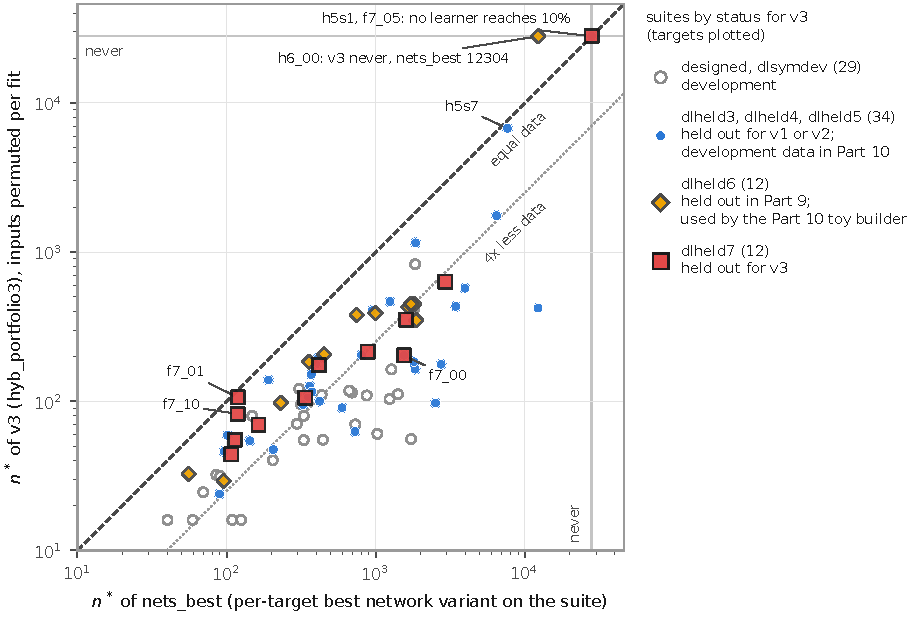
\includegraphics[width=\linewidth]{figures/fig_toy_nstar.pdf}
\caption{$\nstar$ of v3 (inputs permuted per fit) against \code{nets_best} for every target of every toy suite with network references, one point per target \status{Numerical}. Colour and shape give the status of the suite for v3 (\cref{tab:status}); the held-out suite \code{dlheld7} is drawn as large outlined squares. ``never'': 10\% error not reached by $n=16384$, drawn at the edge. Points below the dashed line need less data than the best network variant, and points below the dotted line at least $4\times$ less. \code{nets_best} is a minimum over 2 variants on \code{designed}, \code{random}, \code{dlheld} and \code{dlheld2}, 3 on \code{dlsymdev} and \code{dlheld3}--\code{dlheld5}, 5 on \code{dlheld6} and the 3 pre-registered ones on \code{dlheld7}. \code{dlfamdev} has no network runs and is not shown. Source: \repo{study/part10/LEARNER_RESULTS.json}.}
\label{fig:toy-nstar}
\end{figure}

\Cref{tab:toy-suites} summarizes all 11 suites, and \cref{fig:toy-nstar} shows every target with a network reference. \Cref{tab:status} gives each suite's status for v3: only \code{dlheld7} is held out, and the footnotes of \cref{tab:toy-suites} mark the suites that shaped v3 or an earlier version.

\paragraph{Results} \status{Numerical}. On the 126 targets of \cref{fig:toy-nstar}, v3 is clearly better than \code{nets_best} on 121 and needs at least $4\times$ less data on 54 (\texttt{figures/fig\_toy\_nstar.json}). Five targets are not wins:
\begin{itemize}
\item h6\_00 (\code{dlheld6}) is clearly worse: only the most regularized network learns it, at 12304;
\item f7\_01 (\code{dlheld7}) and h5s7 (\code{dlheld5}) are ties;
\item f7\_05 (\code{dlheld7}) and h5s1 (\code{dlheld5}) are learned by no learner.
\end{itemize}
\Cref{sec:res-toy-fail} discusses them. The suite means against \code{nets_best} range from $-1.50$ to $-2.44$ (\cref{tab:toy-suites}).

\paragraph{Against the one variant run on every suite} \status{Numerical}. The suite means against \code{nets_best} are not comparable across suites, because \code{nets_best} minimizes over different sets of variants. \code{nets_wd} is the one variant run on every suite with network results. Against it, v3's mean $\log_2\nstar$ ratio is:
\begin{itemize}
\item development suites: $-2.42$ on \code{designed} and $-2.53$ on \code{dlsymdev}; the Part 6 development check \code{random}: $-2.26$;
\item earlier held-out suites: $-2.03$ on \code{dlheld}, $-1.99$ on \code{dlheld2}, $-2.07$ on \code{dlheld3}, $-2.25$ on \code{dlheld4} and $-2.66$ on \code{dlheld5};
\item the two draws of the blind family: $-1.94$ on \code{dlheld6} and $-1.83$ on \code{dlheld7}.
\end{itemize}
The two draws of the blind family give the two smallest margins, but \code{dlheld2} is within 0.05 of \code{dlheld6}, and differences of this size on suites of 7 to 12 targets are within noise. If the gap is real, two explanations fit it, and the data do not separate them \status{Heuristic}. Several of the other suites informed the design of v3 or of an earlier version, so some selection in v3's favour is expected there. And the suites differ in kind: \code{dlheld}--\code{dlheld5} were written within the study, mostly from families close to its development targets, while the blind family was written by an agent that had not seen the sum-feature design.

\paragraph{Wins that need no feature search, over the held-out suites} \status{Numerical}. Excluding the 30 of the 77 targets of the seven held-out suites (\code{dlheld}--\code{dlheld7}) on which \code{lin} or \code{hgb} is already clearly better than \code{nets_best}, v3's mean against \code{nets_best} is $-2.11$ over the 44 that both learn, with 42 targets clearly better and 1 clearly worse (\texttt{figures/fig\_toy\_nstar.json}). The 30 are of two kinds: 6 halfspace-like targets on which \code{lin} wins (v3 is within the tie band of \code{lin} or below it on each), and 24, mostly formulas, decision lists, multiplexers and controls, on which \code{hgb} wins; \cref{app:further-toy} lists them. So the margins do not come from targets that are easy for trees or linear models. They come from the targets with parity or signed-sum structure, where both calibration references fail, and Part 8's ablations located the toy wins in DFG \cite{discretelearners2026}. The pooled summary over the seven held-out suites, most of them development data for v3, is in \cref{app:further-toy}.

% ------------------------------------------------------------------------------------------------------------------
\subsection{Where v3 is not better}\label{sec:res-toy-fail}

Five of the 126 targets with network references are not wins (\cref{fig:toy-nstar}).
\begin{itemize}
\item \emph{Learned by no learner.} f7\_05 $=[\tfrac12(s+14)\bmod3\ne0]$, $s=x_1+\dots+x_{14}$ (\code{dlheld7}), and h5s1, a signed 9-input count with accept set $\{-9,-5,-1,3,9\}$ times the parity $x_{10}x_{11}$ (\code{dlheld5}). No network variant, \code{lin} or \code{hgb} reaches 10\% error on either by $n=16384$ (3 seeds).
\item \emph{The one loss.} h6\_00, a residue class mod 3 of a 13-input count (\code{dlheld6}), is learned only by the most regularized network (\code{nets_cewd1.0}, $\nstar=12304$). It is the only target of any suite on which a network is clearly better than v3, and it was v2's loss as well. The third residue class mod 3, fd\_10 on 10 inputs (\code{dlfamdev}), has no network runs. v3 and v2 learn none of the three by $n=16384$.
\item \emph{Ties.} The halfspace f7\_01 $=[x_1+\dots+x_{13}\le1]$: v3 (106), \code{lin} (111) and the logistic-loss networks (119--121) are all within the tie band, and a linear readout of the inputs alone already does about as well. And h5s7, an arbitrary accept set of a signed 13-input count: 6760 against 7641 (\code{nets_cewd}).
\end{itemize}
The interpretability analysis (seed 0) locates the failures on the residue classes in DFG's search, not in its test: their true blocks would pass the test from $n=128$, but the targets have almost no Fourier weight at degrees 1--2, from which every seed of the search starts (\cref{sec:interp-toy-fail}; \cref{sec:dfg} explains why such a block is invisible to the seeds). h5s7 is a weaker case of the same mechanism, found at $n=8192$ on seed 0, and h5s1's bottleneck is detecting its modulating parity (\cref{app:interp-late}). The next-smallest margins are listed in \cref{app:further-toy}.

% ------------------------------------------------------------------------------------------------------------------
\subsection{Tabular data}\label{sec:res-tabular}

\paragraph{What v3 runs on tabular data.} DFG runs only when there are 2 classes and every column is binary or categorical ($\le256$ bits), and the image members only on images. So on 24 of the 26 datasets v3 runs v1's code, the stack of LightGBM, ExtraTrees, $k$-NN and logistic regression (its predictions were checked identical to v2's on one optdigits fit, and v2 runs v1's code path there), and its results there are v1's Part 8 result files. Only two datasets qualify for DFG: kr\_vs\_kp (development) and mushroom (Part 7 held-out set). On mushroom v3's own runs give v1's seed-mean errors at every $n$. On kr\_vs\_kp they differ from v1's at 3 of 4 sizes, but at no cell clearly (\cref{app:further-tab}).

\paragraph{What is held out.} HELDOUT2 (10 datasets) was fixed in a commit before any Part 8 design work (\texttt{04a215b2}). v1 was developed on the 5 development datasets only, and its code path has not changed since. HELDOUT2 contains no dataset on which DFG runs, so it is held out for this code path. The Part 7 held-out set is held out in the weaker sense that the Part 8 designers had read its MLP references. The 5 development datasets are in-sample.

\begin{table}[t]
\centering{\footnotesize\setlength{\tabcolsep}{4pt}
\begin{tabular}{llccc}
\toprule
split & reference & cells (better / tie / worse) & mean $\log_2$ ratio & datasets lower (sign test $p$)\\
\midrule
Part 7 held-out set & \code{mlp} & 59 (22/36/1) & $-0.331$ & 10 of 11 (0.012)\\
 & \code{mlp_reg} & 59 (16/40/3) & $-0.160$ & 9 of 11 (0.065)\\
 & \code{mlp_strong} & 54 (22/30/2) & $-0.339$ & 10 of 11 (0.012)\\
 & \code{mlp_best} & 59 (12/44/3) & $-0.114$ & 8 of 11 (0.23)\\
 & \code{hgb} & 59 (20/38/1) & $-0.259$ & 10 of 11 (0.012)\\
\midrule
Part 8 fresh set (HELDOUT2) & \code{mlp} & 53 (15/36/2) & $-0.445$ & 9 of 10 (0.021)\\
 & \code{mlp_reg} & 53 (16/35/2) & $-0.272$ & 8 of 10 (0.11)\\
 & \code{mlp_strong} & 53 (15/36/2) & $-0.284$ & 8 of 10 (0.11)\\
 & \code{mlp_best} & 53 (10/41/2) & $-0.168$ & 8 of 10 (0.11)\\
 & \code{hgb} & 53 (12/40/1) & $-0.250$ & 9 of 10 (0.021)\\
\midrule
development & \code{mlp} & 24 (4/20/0) & $-0.379$ & 5 of 5 (0.062)\\
 & \code{mlp_reg} & 24 (3/21/0) & $-0.267$ & 5 of 5 (0.062)\\
 & \code{mlp_best} & 24 (1/23/0) & $-0.244$ & 5 of 5 (0.062)\\
 & \code{hgb} & 24 (4/20/0) & $-0.270$ & 5 of 5 (0.062)\\
\bottomrule
\end{tabular}
}
\caption{v3 on the tabular datasets against the MLP references and \code{hgb} \status{Numerical}. ``Cells'': the $(\text{dataset},n)$ pairs compared, each a mean over 3 seeds, with the verdict rule of \cref{sec:metrics}. ``Mean $\log_2$ ratio'': of v3's test error to the reference's, over cells, errors floored at 0.002. The last column counts the datasets whose mean ratio over $n$ is below 0, with the two-sided sign-test $p$. \code{mlp_best} is the per-cell best of the Part 7--8 MLP variants (hindsight). \code{mlp_strong} was run on the Part 7 set only at $n\le10000$ (54 of 59 cells) and not on the development sets. On 24 of the 26 datasets v3's code path is v1's, so these are Part 8's numbers, except for v3's own runs on mushroom (identical errors) and kr\_vs\_kp. Source: \repo{study/part10/LEARNER_RESULTS.json}.}
\label{tab:real}
\end{table}

\paragraph{Results} (\cref{tab:real}) \status{Numerical}.
\begin{itemize}
\item \emph{HELDOUT2, against \code{mlp_best}:} mean $\log_2$ error ratio $-0.168$, a geometric-mean error about 11\% lower. 10 of 53 cells are better and 2 worse. The mean error is lower on 8 of 10 datasets, which is not significant (sign test $p=0.11$).
\item \emph{HELDOUT2, against single references:} the margins are larger: $-0.445$ against the baseline \code{mlp} (9 of 10 datasets, $p=0.021$), $-0.284$ against \code{mlp_strong} (8 of 10, $p=0.11$) and $-0.250$ against \code{hgb} (9 of 10, $p=0.021$).
\item \emph{The Part 7 set:} $-0.114$ against \code{mlp_best} (12 better, 3 worse, 8 of 11 datasets, $p=0.23$) and $-0.259$ against \code{hgb} (10 of 11, $p=0.012$).
\item \emph{Development:} $-0.244$ against \code{mlp_best}, lower on 5 of 5 ($p=0.062$).
\end{itemize}
The per-dataset picture is in \cref{app:further-tab}.

\paragraph{Where the tabular result comes from} \status{Heuristic}. The tabular numbers are those of a classical stack, and they say little about discrete feature search: in Part 8, DFG did not carry them, no single member family matched the stack, and default \code{hgb} alone did not beat the MLPs \cite{discretelearners2026} (\cref{app:further-tab}). This agrees with the tabular-learning literature. Tree ensembles tend to beat plain MLPs on medium-sized tabular data \cite{grinsztajn2022tree,shwartzziv2022tabular}. Stacking diverse models adds to that \cite{wolpert1992stacked,erickson2020autogluon}. And careful regularization and tuning of the MLP narrow the gap \cite{kadra2021welltuned,gorishniy2021revisiting}. The MLP references here are standard recipes without tabular-specific architectures, so the margins would likely shrink against a tuned tabular network \status{Heuristic}. The tabular evidence for v3 is therefore modest: it is not worse than the MLPs on average on fresh tabular data (2 of 10 datasets have higher mean error), it is better on average without statistical significance, and the reason is the classical stack, unchanged since Part 8.
